\part{Développements avec Python}
\label{part:dev_Python}

\section{Généralités}
Les développements sont en \textbf{\texttt{Python3}} et rassemblés dans le
répertoire : \\
\-\hspace{1cm} \path{$AIDA_HOME/src/python3}.
\smallbreak

  Le code est indenté par 4 espaces (et non pas le caractère TAB). Il peut être
nécessaire de régler votre éditeur préféré afin qu'il insère 4 espaces lorsque
la touche TAB est tapée.
\smallbreak

  Les codes python doivent débuter par le sheebang :
\begin{boxedverbatim}
#!/usr/bin/env python3
\end{boxedverbatim}
\smallbreak

La documentation, générée par \texttt{sphinx}, est sous : \\
\-\hspace{1cm} \path{$AIDA_HOME/doc/sphinx/html/index.html}.

\section{Règles de codages}
   Il est vivement conseillé de suivre les conventions de codage usuelles du
monde Python, formalisées dans le PEP-8
\footnote{\url{http://www.python.org/dev/peps/pep-0008/}},
et vérifiables par pylint\footnote{\url{http://www.pylint.org/}}.
\smallbreak

  Le code écrit pour AIDA doit être (autant que faire se peut) indépendant de
la plateforme. En particulier, la construction des noms de répertoire et de
fichier doit être faite en utilisant la méthode \textbf{\texttt{os.path.join}}.
En aucun cas le séparateur \texttt{/} ne doit être explicitement utilisé.
\smallbreak

  En aucun cas la variable d'environnement \texttt{PYTHONPATH} ne doit être
utilisée, que ce soit de façon implicite ou explicite
(voir : \nameref{sec:import_AIDA}, page \pageref{sec:import_AIDA}). \\
\smallbreak

Il est vivement recommandé de coder un \textit{main} dans les modules afin de
permettre de \textbf{tester le code} :
\begin{boxedverbatim}
if __name__ == '__main__':
\end{boxedverbatim}


\section{Les modules de AIDA}
  Les modules de \textbf{AIDA} rassemblent les outils (fonctions, classes)
utiles pour travailler dans un environnement AIDA. Ils sont regroupés sous le
répertoire : \\
\-\hspace{1cm} \path{$AIDA_HOME/src/python3/AIDA_lib}

\medbreak
\textbf{Afin de faciliter la maintenance du code AIDA, ces modules
doivent être utilisés par les programmes développés dans le cadre du projet}.

\subsection{Utilisation des modules de AIDA}
\label{sec:import_AIDA}
  Tout programme souhaitant utiliser les modules de AIDA doit modifier
\textbf{explicitement} la variable de recherche des modules avant d'importer
les modules désirés.
Le système d'installation de AIDA copie les modules dans le répertoire : \\
\-\hspace{1cm} \path{$AIDA_HOME/lib/python<num_version>}. \\
Ce sont ces copies qui doivent être importées par l'utilisation du code
suivant :

\medbreak
\begin{boxedverbatim}
import os
import sys

PYTHON_X_Y = 'python%d.%d' % (sys.version_info[0], sys.version_info[1])
sys.path.append(os.path.join(os.getenv('AIDA_HOME'), 'lib', PYTHON_X_Y))

import ...

\end{boxedverbatim}

\subsection{Documentation des modules de AIDA}
  Afin que la documentation d'un module de AIDA apparaise dans la documentation
générale, il convient de la faire générer par \texttt{sphinx}. \\
Pour cela, il suffit d'ajouter une section au fichier : \\
\-\hspace{1cm} \path{$AIDA_HOME/src/doc/sphinx/source/modules_python.rst}


\subsection{Le module \emph{AIDA.py}}
  Les éléments principaux sont :
  \begin{itemize}
    \item[•] La classe Vector
    \item[•] La classe Inf
    \item[•] des fonctions liées aux conventions AIDA
      \subitem - \texttt{Y2\_to\_Y4},
      \subitem - \texttt{AIDA\_freq\_fmt},
      \subitem - \texttt{AIDA\_abrev\_to\_family},
      \subitem - \texttt{AIDA\_abrev\_to\_plt},
      \subitem - \texttt{AIDA\_long\_to\_abrev}
    \item[•] des fonctions d'utilisation des indicateurs d'acquisition
      \subitem - \texttt{ID\_to\_full},
      \subitem - \texttt{ID\_to\_relpath},
      \subitem - \texttt{ID\_to\_datapath},
      \subitem - \texttt{ID\_to\_infpath},
  \end{itemize}

  Voir la documentation complète :  \\
\-\hspace{1cm} \path{$AIDA_HOME/doc/sphinx/html/index.html}.


\section{Écriture d’un opérateur}
\label{sec:adc_oper}

  Pour des raisons historiques, un opérateur, dans l'environnement AIDA, peut
être de deux natures :
  \begin{itemize}
    \item[•] codé en Python
    \item[•] codé en C
             (voir \nameref{sec:ecr_oper}, page \pageref{sec:ecr_oper}).
  \end{itemize}

\medbreak
  Un opérateur a pour vocation d'être appelé par l'interpréteur de commande de
AIDA : \texttt{adc}. Cependant, il pourrait être appelé par tout autre
programme utilisant la même interface d'appel. Dans la suite de cette
documentation le seul vocable \texttt{adc} sera utilisé.

\medbreak
  Un opérateur Python est constitué de 4 parties :
  \begin{itemize}
    \item[•] une fonction de caclul.
    \item[•] une fonction d'interface entre la fonction de calcul et
             \texttt{adc}.
    \item[•] une description de la fonction d'interface.
    \item[•] une documentation.
  \end{itemize}

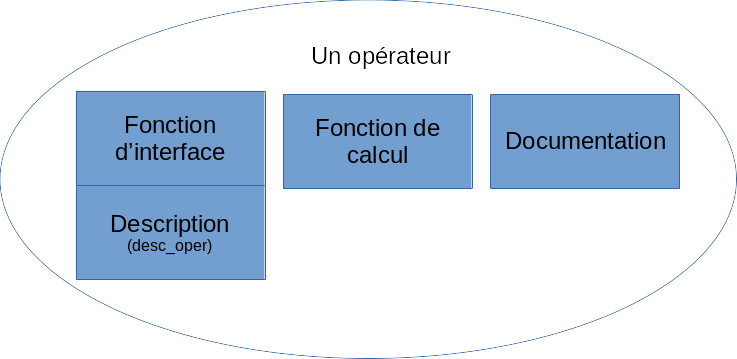
\includegraphics[scale=0.5]{images/schema_oper.png}

\subsection{une fonction de caclul}
  C'est une fonction Python qui effectue un traitement sur une série
  temporelle de données : les données d'un vecteur. \\

  Généralement elle reçoit les données des séries temporelles et retourne ses
  résultats sous forme de tableaux \texttt{numpy}. \\

  Les fonctions de calcul sont regroupées sous : \\
  \-\hspace{1cm} \path{$AIDA_HOME/src/python3/packages/calcul}.  \\

  (voir : \nameref{sec:ex_fct_calcul}, page \pageref{sec:ex_fct_calcul}). \\

  Si le code du module contient un \textit{main}, son code doit permettre de
  \textbf{tester la fonction de calcul}.


\subsection{une fonction d'interface}
  C'est une fonction Python qui fait l'interface entre la fonction de calcul
  et \texttt{adc}. \\

  Ses paramètres d'entrée sont des objets AIDA \textbf{\texttt{VectorMask}},
  des \textbf{\texttt{coefficients}}. \\

  Cette fonction Python peut déclarer des paramètres optionnels selon les
  principes de la programmation Python. \\

  Le code de la fonction d'interface est divisé en 4 phases :
  \begin{itemize}
    \item[•] préparation des arguments pour appeller la fonction de calcul.
    \item[•] appel de la fonction de calcul.
    \item[•] préparation du/des header(s) du/des vecteur(s) de retour.
    \item[•] préparation du diagnostique d'exécution.
  \end{itemize}
\medbreak

  Elle retourne ses résultats sous la forme d'un tuple :
  \begin{itemize}
    \item[•] liste des headers
    \item[•] liste des données
    \item[•] dictionnaire du diagnostique
    \subitem - clé 'CodeRet' : int(),
    \subitem - clé 'DiagExec': string()
  \end{itemize}
\medbreak

  Les fonctions d'interface sont regroupées sous : \\
  \-\hspace{1cm} \path{$AIDA_HOME/src/python3/packages/oper}. \\

  (voir : \nameref{sec:ex_fct_interface}, page \pageref{sec:ex_fct_interface}). \\

  Si le code du module contient un \textit{main}, son code doit permettre de
  \textbf{tester la fonction d'interface}.


\subsection{une description de la fonction d'interface}
  Cette description permet d'unifier pour \texttt{adc} l'appel des
  différents opérateurs. \\
  Elle permet également à \texttt{adc} d'effectuer des contrôles de cohérence
  entre la ligne de commande reçue et les attendus de l'opérateur. \\
  \textbf{\textit{Note : par abus de langage, cette fonction d'interface est
                  souvent nommée : \textit{l'opérateur}. }} \\

  Cette description est faite dans le fichier de la fonction d'interface
  (\path{$AIDA_HOME/src/python3/packages/oper}) \\
  C'est un dictionnaire Python de nom \textbf{\texttt{desc\_oper}} dont la
  forme générale est :
  \medbreak

  \begin{boxedverbatim}
    desc_oper = {
        '<Nom de l'opérateur>': {
            'Args': [
                {'Id'       : '<param>',
                 'categorie': '<catégorie>'
                 'unit'     : '<unité>',
                 'famille'  : ['<famille_1>', '<famille_2>', ...]
                },
                ..
            ],
        '<directive>': '<valeur>',
        },
    }
  \end{boxedverbatim}
  \medbreak

  (voir : \nameref{sec:ex_fct_interface}, page \pageref{sec:ex_fct_interface}). \\

  Ce dictionnaire (\textbf{\texttt{desc\_oper}}) décrit, pour un opérateur
  (\textbf{\texttt{<Nom de l'opérateur>}}) :
  \begin{itemize}
    \item[•] ses paramètres d'entrée, dans l'ordre attendus par la fonction
             d'interface. \\
             (voir : \nameref{sec:param_in}, page \pageref{sec:param_in})
    \item[•] ses paramètres de sortie, dans l'ordre des retours de la fonction
             d'interface. \\
             (voir : \nameref{sec:param_out}, page \pageref{sec:param_out})
    \item[•] des directives de traitement modifiant le comportement par défaut
             de \texttt{adc}. \\
             (voir : \nameref{sec:directives}, page \pageref{sec:directives}) \\
             \textbf{\textit{Ces directives sont optionnelles. }}
  \end{itemize}
  \medbreak

  Les paramètres \textbf{optionnels} de la fonction d'interface
  \textbf{ne sont pas décrits} dans le dictionnaire
  \textbf{\texttt{desc\_oper}}
  \medbreak

  Les paramètres d'entrée et de sortie de la fonction d'interface sont décrits
  dans la clé \textbf{\texttt{'Args'}} du dictionnaire
  \textbf{\texttt{<desc\_oper>}}. Cette clé est une
  \textit{liste de dictionnaires} : chacun de ces dictionnaires décrit un
  argument. \\

  Les directives de traitement sont déclarées dans des clés spécifiques du
  dictionnaire \textbf{\texttt{<desc\_oper>}}.
  \medbreak

  \medbreak

\subsubsection{description des paramètres d'entrée de la fonction d'interface}
\label{sec:param_in}
Chaque paramètre d'entrée de la fonction d'interface doit être décrit par
un dictionnaire dans la clé \textbf{\texttt{'Args'}} du dictionnaire
\textbf{\texttt{desc\_oper}} , dans l'ordre attendu par la fonction
d'interface. \\

La forme générale du dictionnaire de descritption d'un paramètre d'entrée est :
  \medbreak

  \begin{boxedverbatim}
    {'Id'       : '<param>',
     'categorie': '<catégorie>'
     'unit'     : '<unité>',
     'famille'  : ['<famille_1>', '<famille_2>', ...]
    },
  \end{boxedverbatim}
  \medbreak

  avec:
  \begin{itemize}
    \item[•] <param> : nom du paramètre d'entrée utilisé dans la fonction
             d'interface.
    \item[•] <catégorie> : catégorie du paramètre parmis :
      \begin{itemize}
      \item \texttt{VECTOR\_IN}  : le paramètre est un vecteur d'entrée.
      \item \texttt{COEFFICIENT} : le paramètre est un coefficient (d'entrée).
      \end{itemize}
  \end{itemize}
  \medbreak

  Les clés \textbf{\texttt{'unit'}} et \textbf{\texttt{'famille'}} sont
  optionnelles. Elles ne peuvent être fournies que pour un paramètre de
  catégorie \textbf{\texttt{VECTOR\_IN}}.
  \medbreak

  Si la clé \textbf{\texttt{'unit'}} est fournie :
  \begin{itemize}
    \item[•] sa valeur (\textbf{\texttt{<unité>}}) doit être une chaîne de
             caractères
    \item[•] sa valeur (\textbf{\texttt{<unité>}}) doit être conforme aux
             unités AIDA \\
             (voir \path{$AIDA_HOME/src/python3/AIDA_lib/Units.py}).
    \item[•] \texttt{adc} transmettra à l'opérateur des données converties
             dans cette unité (si possible et si besoin). \\
             Ex : si les données du vecteur d'entrée sont en \texttt{Celsius}
             mais que description du paramètre spécifie \texttt{'unit': 'K'},
             alors \texttt{adc} convertira les données reçues de
             \texttt{Celsius} en \texttt{kelvin} avant de transmettre les
             données à l'opérateur (le vecteur d'entrée sur disque n'est pas
             modifié).
  \end{itemize}
  \medbreak

  Si la clé \textbf{\texttt{'famille'}} est fournie :
  \begin{itemize}
    \item[•] sa valeur doit être une liste de chaîne de caractères
    \item[•] chacune des chaînes de caractères de la liste  doit être le nom
             d'une famille AIDA  \\
             (voir \path{$AIDA_HOME/config/familles}).
    \item[•] \texttt{adc} vérifiera, avant d'appeler l'opérateur, que le
             vecteur d'entrée fourni est bien de l'une des familles de la liste.
             Dans le cas contraire, \texttt{adc} s'arrêtera en erreur. Ce
             comportement \texttt{adc} peut être supprimer par l'utilisation de
             l'option \texttt{-C} au lancement d'\texttt{adc}. \\
  \end{itemize}

\subsubsection{description des paramètres de sortie de la fonction d'interface}
\label{sec:param_out}
Chaque paramètre de sortie de la fonction d'interface doit être décrit par
un dictionnaire dans la clé \textbf{\texttt{'Args'}} du dictionnaire
\textbf{\texttt{desc\_oper}} , dans l'ordre des retour de la fonction
d'interface. \\

La forme générale du dictionnaire de descritption d'un paramètre de sortie est :
  \medbreak

  \begin{boxedverbatim}
    {'Id': '<param>', 'categorie': 'VECTOR_OUT'},
  \end{boxedverbatim}
  \medbreak

  avec:
  \begin{itemize}
    \item[•] <param> : nom du paramètre de sortie utilisé dans la fonction
             d'interface.
    \item[•] <catégorie> : la chaîne de caractère \texttt{'VECTOR\_OUT'}.
  \end{itemize}
  \medbreak

\subsubsection{description des directives de traitement}
\label{sec:directives}
Chaque directive de traitement doit être décrite par une clé du dictionnaire
\textbf{\texttt{desc\_oper}}.

La forme générale de description d'une directive de traitement est :
  \medbreak

  \begin{boxedverbatim}
    '<directive>': '<valeur>'
  \end{boxedverbatim}
  \medbreak

  Les directives de traitement possibles sont :
  \begin{itemize}
    \item[•] \textbf{\texttt{control\_reftime}} \\
             Sa valeur peut être : \texttt{'on'} ou \texttt{'off'}. \\
             Sa valeur par défaut est : \texttt{'on'}. \\
             Lorsque cette clé est à \texttt{'on'}, \texttt{adc} contrôle que
             toutes les séries temporelles ont des bases de temps équivalentes
             (champ \texttt{'ref\_time'} des vecteurs) avant d'appeler la
             fonction d'interface de l'opérateur. \\

             Lorsque cette clé est à \texttt{'off'}, \texttt{adc} ne fait aucun
             contrôle sur la cohérence des bases de temps des séries
             temporelles avant d'appeler la fonction d'interface de l'opérateur. \\

             Concrètement, seuls les opérateurs modifiant les données en
             fonction d'une autre base de temps (ex \texttt{Ech\_tps\_impos})
             positionnent ce contrôle à \texttt{'off'}. \\

    \item[•] \textbf{\texttt{repl\_oper}}
    \item[•] \textbf{\texttt{repl\_cause}} \\
             Ces 2 directives marchent de paire. Elles précisent que cet
             opérateur est obsolète. \\

             La valeur de la directive \texttt{repl\_oper} est alors le nom du
             nouvel opérateur à utiliser. \\

             La valeur de la directive \texttt{repl\_cause} précise la raison
             pour laquelle cet opérateur a été remplacé. \\

             Lors de l'appel d'un opérateur dont la description précise ces
             2 clés, \texttt{adc} affiche un message d'obsolescence. \\

             Ex : la description de l'opérateur Mon\_operateur contient :

             \begin{boxedverbatim}
        'repl_oper' : 'new_oper',
        'repl_cause': 'Mon_operateur ne permet pas de faire xxx',
             \end{boxedverbatim}

             A l'utilisation de cet opérateur, \texttt{adc} affiche :

             \begin{boxedverbatim}
        -+- L'operateur Mon_operateur est obsolete : remplacez-le par new_oper
        -+- cause : Mon_operateur ne permet pas de faire xxx
             \end{boxedverbatim}
  \end{itemize}


\subsection{une documentation}

  La documentation des opérateurs est dans le répertoire : \\
  \-\hspace{1cm} \path{$AIDA_HOME/src/doc/oper}. \\

  (voir : \nameref{sec:ex_doc_oper}, page \pageref{sec:ex_doc_oper}). \\

  Elle est écrite en \LaTeX{} et peut être éditée avec des éditeurs
généralistes (vi, emacs) ou spécialisés (TexMaker, ...).

  La plupart du temps, il n'est pas nécessaire d'être expert en
\LaTeX{} pour écrire la documentation. Si besoin est, une
rapide introduction à l'écriture de mathématiques en
\LaTeX{}  se trouve sur le site des tuteurs de l'ENS :
\url{http://www.tuteurs.ens.fr/logiciels/latex/maths.html}.
Il faut être attentif à quelques points :

\begin{itemize}
  \item les noms des variables utilisés dans la formule doivent correspondre
    aux noms donnés dans la liste des arguments.
  \item il ne faut pas utiliser la commande
    \clavier{\textbackslash\textbackslash} pour forcer un changement de ligne
    de texte : les méthodes recommandées sont d'utiliser le mode math
    hors-texte (\verb+\[ ... \]+), ou le changement de paragraphe canonique
    (ligne vide).
\end{itemize}

\medbreak
  La documentation d'un opérateur est répartie en trois fichiers. Le premier
(document principal) inclue les 2 autres :

\medbreak
\begin{description}
  \item[{\path{Mon_Oper.tex}}] : \\
    Ce fichier contient la description de l'opérateur.

  \item[{\path{arguments/Mon_Oper.args.tex}}] : \\
    Ce fichier contient la description des arguments de l'opérateur.

    \begin{description}
      \item Les arguments d'entrée sont décrits dans le tableau dont le nom
            est : \\
            \texttt{Entrées}.

      \item Les arguments de sortie sont décrits dans le tableau dont le nom
            est : \\
            \texttt{Sorties}.
    \end{description}

    La forme générale de description d'un argument d'entrée ou de sortie est :

    \begin{boxedverbatim}
        $nom$ & type, format & description\\
    \end{boxedverbatim}

    avec type   = Vecteur ou Coef. \\
    et   format = float, double, int, string...


    \begin{description}
      \item Les arguments optionnels sont décrits dans le tableau dont le nom
            est : \\
            \texttt{Entrées optionnelles}.
    \end{description}

    La forme générale de description d'un argument d'entrée ou de sortie est :

    \begin{boxedverbatim}
        $nom$ & format & description\\
    \end{boxedverbatim}

    avec format = NUM, list(), dict(), bool(), str(). \\
    Lorsque le format est NUM, le paramètre fournit à l'appel doit être de
    type numérique (int, float).

    \textbf{\textit{Note : la balise \texttt{hline} doit être présente une
                    fois et une seule par tableau.}} \\

  \item[{\path{formules/Mon_Oper.frm.tex}}] : \\
    Ce fichier contient la formule de calcul de l'opérateur (il est
    facultatif). \\
    Une version anglaise peut être présente : elle sera écrite dans le fichier
    \path{formules/Mon_Oper.frm.en.tex}
\end{description}



  Après avoir écrit les fichiers de la documentation d'un opérateur, il faut :

  \begin{itemize}
    \item[•] modifier le fichier \pathfmt{CATALOG_OPER.tex} pour ajouter les deux
      lignes suivantes dans le chapître adapté : \\
      \begin{boxedverbatim}
\input{Mon\_Oper}
\newpage \end{boxedverbatim}

    \item[•] produire la nouvelle version de \pathfmt{CATALOG_OPER.pdf} par la
        commande : \fbox{\texttt{make CATALOG.pdf}}.

    \item[•] itérer les actions d'édition/compilation/relecture jusqu'à
      satisfaction

    \item[•] tester si la documentation qui vient d'être écrite est bien
      utilisable pour générer la documentation automatique d'un traitement.
      Voir \texttt{mk\_doctrt} (\url{user.pdf})

    \item[•] enregistrer toutes les modification dans le système de gestion de
      code (\texttt{git})
  \end{itemize}

\medbreak
  Il n'est jamais nécessaire de créer ces trois fichiers \texttt{.tex}
\textit{ex nihilo}. Si l'opérateur que l'on vient de créer ressemble à un
opérateur existant, il suffira de copier et modifier les fichiers de cet
opérateur \textbf{en prenant soin d'adapter les balises}. Sinon, deux
programmes permettent de créer un squelette de documentation :

\begin{description}
  \item[\texttt{oper2doc}] : \\
     Génère un squelette de documentation pour les opérateurs C.
     Le code source et l'exécutable de ce programme se trouve dans le
     répertoire \path{$AIDA_HOME/src/lib/oper}

  \item[\texttt{oper\_py\_2doc.py}]:  \\
     Génère un squelette de documentation pour les opérateurs Python.
     L'exécutable de ce programme est installé dans \path{$AIDA_HOME/bin}. \\
     La commande \fbox{\texttt{oper\_py\_2doc.py -h}} permet d'afficher l'aide
     de ce programme.
\end{description}

\newpage
\subsection{Concrètement}
  L'opérateur \textit{Mon\_Oper} sera le résultat des
  \textbf{cinq fichiers} : \\

  \begin{description}
    \item[•] \path{$AIDA_HOME/src/python3/packages/calcul/Mon_Oper.py}
    \item[•] \path{$AIDA_HOME/src/python3/packages/oper/Mon_Oper.py}
    \item[•] \path{$AIDA_HOME/src/doc/oper/Mon_Oper.tex}
    \item[•] \path{$AIDA_HOME/src/doc/oper/arguments/Mon_Oper.args.tex}
    \item[•] \path{$AIDA_HOME/src/doc/oper/formules/Mon_Oper.frm.tex}
  \end{description}

  Ci-après, sont présentés des squelettes de ces 5 fichiers.

\subsubsection{exemple de fonction de calcul}
\label{sec:ex_fct_calcul}
\path{$AIDA_HOME/src/python3/packages/calcul/Mon_Oper.py} :

  \begin{boxedverbatim}
  def Mon_Oper(P, T, coef):
      """
      Fonction de calcul de X en fonction de P, T et coef.

      Input :
        P    : pression
        T    : température
        coef : coefficient...

      Outut :
        X    : résultat...
      """
      ...

      return X
  \end{boxedverbatim}


\subsubsection{exemple de fonction de d'interface et de sa description}
\label{sec:ex_fct_interface}
\path{$AIDA_HOME/src/python3/packages/oper/Mon_Oper.py} :

  \begin{boxedverbatim}
  def Mon_Oper(P, T, coef, limits={'min': 0, 'max': 100}):
      """ Fonction d'interface de l'opérateur Mon_Oper.
          Cet opérateur calule X en fonction de P, T et coef, en fonction de limits.

          Input :
              P    : ...
              T    : ...
              coef : ...
              limits : (paramètre optionnel) limitation ...

        Output :
              X    : ...
      """
      # récupération des arguments
      P_header = P.attributes
      P_data   = P.data.data

      T_header = T.attributes
      T_data   = T.data.data

      # préparation des arguments pour la fonction de calcul
      ...

      # appel de la fonction de calcul
      X = calcul.Mon_Oper.Mon_Oper(P_data, T_data, coef, limits)

      # préparation du retour
      X_header = ...
      ...

      # diagnostique
      diag = {'CodeRet' : 0,
              'DiagExec': f"Mon_oper : ({len(P_data)} ech.), " + ...
             }

      # retour
      return [X_header], [X_data], diag

  # Description de l'opérateur
  desc_oper = {
    'Mon_Oper': {
      'Args': [
        {'Id'       : 'P'         ,
         'categorie': 'VECTOR_IN' ,
         'unit'     : 'hPa'       ,
         'famille'  : ['pression']
        },
        {'Id': 'T'   , 'categorie': 'VECTOR_IN'                  },
        {'Id': 'coef', 'categorie': 'COEFFICIENT'                },
        {'Id': 'X'   , 'categorie': 'VECTOR_OUT'                 },
      ],
      'control_reftime': 'on', # valeur par défaut => précision inutile
    },
  }
  \end{boxedverbatim}

\subsubsection{exemple de documentation}
\label{sec:ex_doc_oper}
\path{$AIDA_HOME/src/doc/oper/Mon_Oper.tex} :

  \begin{boxedverbatim}
  \section{Un titre de section}

  \itemstyle{Op\'erateur~:} \operfmt{Mon\_Oper}
  \index{Mon\_Oper}

  %%%%%OBJET%%%%
  \itemstyle{Objet~:}
  Explications...

  %%%%%ARGUMENTS%%%%
  \bigskip
  \input{arguments/Mon_Oper.args.tex}

  %%%%%FORMULE%%%%
  \itemstyle{Formule}

  \input{formules/Mon_Oper.frm.tex}

  %%%%%AUTEUR%%%%
  \itemstyle{Auteur~:}
  CNRM/GMEI/TRAMM

  %%%%%REFERENCE%%%%
  \itemstyle{R\'ef\'erences~:}
  \end{boxedverbatim}

\smallbreak
\path{$AIDA_HOME/src/doc/oper/arguments/Mon_Oper.args.tex} :

  \begin{boxedverbatim}
  %%%%%ENTREES%%%%
  \begin{tabarg}
  \multicolumn{3}{l}{\titretab {Entrées}}\\
  \hline
  $P_0$ & Vecteur, \texttt{float} &  Pression au niveau $Z_0$ (hPa)\\ 
  ...
  \end{tabarg}
  
  \medskip
  
  %%%%%SORTIES%%%%
  \begin{tabarg}
  \multicolumn{3}{l}{\titretab {Sorties}}\\
  \hline
  $X$ & Vecteur, \texttt{float} & Pression estimée \`a l'altitude Z (hPa)\\
  \end{tabarg}
  
  %%%%%ENTREES OPTIONNELLES%%%%
  \begin{tabarg}
  \multicolumn{3}{l}{\titretab {Entrées optionnelles}}\\
  \hline
  $limits$  & dict()    & Limitation des valeurs. Défaut : "min": 0, "max": 100\\
  \end{tabarg}

\medskip

  \end{boxedverbatim}

\smallbreak
\path{$AIDA_HOME/src/doc/oper/formules/Mon_Oper.frm.tex} :

  \begin{boxedverbatim}
  %% Formule de l'operateur : Mon_Oper
  \[
  ...
  \]
  \end{boxedverbatim}

